%%%%%%%%%%%%%%%%%%%%% chapter.tex %%%%%%%%%%%%%%%%%%%%%%%%%%%%%%%%%
%
% sample chapter
%
% Use this file as a template for your own input.
%
%%%%%%%%%%%%%%%%%%%%%%%% Springer-Verlag %%%%%%%%%%%%%%%%%%%%%%%%%%
%\motto{Use the template \emph{chapter.tex} to style the various elements of your chapter content.}

\chapter{Rosetta Code Tasks starting with G}

\section*{GUI component interaction}

Almost every application needs to communicate with the user in some way.
Therefore, a substantial part of the code deals with the interaction of
program logic with GUI components. Typically, the following is needed:

\begin{itemize}
\item
  put values into input fields under program control
\item
  read and check input from the user
\item
  pop up dialogs to query the user for further information
\end{itemize}

The task: For a minimal ``application'', write a program that presents a
form with three components to the user: A numeric input field
(``Value'') and two buttons (``increment'' and ``random'').

The field is initialized to zero. The user may manually enter a new
value into the field, or increment its value with the ``increment''
button. Entering a non-numeric value should be either impossible, or
issue an error message.

Pressing the ``random'' button presents a confirmation dialog, and
resets the field's value to a random value if the answer is ``Yes''.

(This task may be regarded as an extension of the task \emph{Simple
  windowed application}).


\begin{wideverbatim}

The standard PicoLisp GUI is HTTP based. Connect your browser to
http://localhost:8080 after starting the following script.

#!/usr/bin/picolisp /usr/lib/picolisp/lib.l

(load "@ext.l" "@lib/http.l" "@lib/xhtml.l" "@lib/form.l")

(de start ()
   (and (app) (zero *Number))
   (action
      (html 0 "Increment" "@lib.css" NIL
         (form NIL
            (gui '(+Var +NumField) '*Number 20 "Value")
            (gui '(+JS +Button) "increment"
               '(inc '*Number) )
            (gui '(+Button) "random"
               '(ask "Reset to a random value?"
                  (setq *Number (rand)) ) ) ) ) ) )

(server 8080 "!start")
(wait)

\end{wideverbatim}

\pagebreak{}
\section*{GUI enabling/disabling of controls}

In addition to fundamental \emph{GUI component interaction}, an
application should dynamically enable and disable GUI components, to
give some guidance to the user, and prohibit (inter)actions which are
inappropriate in the current state of the application.

The task: Similar to the task \emph{GUI component interaction} write a
program that presents a form with three components to the user: A
numeric input field (``Value'') and two buttons (``increment'' and
``decrement'').

The field is initialized to zero. The user may manually enter a new
value into the field, increment its value with the ``increment'' button,
or decrement the value with the ``decrement'' button.

The input field should be enabled only when its value is zero. The
``increment'' button only as long as the field's value is less then 10:
When the value 10 is reached, the button should go into a disabled
state. Analogously, the ``decrement'' button should be enabled only as
long as the value is greater than zero.

Effectively, the user can now either increment up to 10, or down to
zero. Manually entering values outside that range is still legal, but
the buttons should reflect that and enable/disable accordingly.


\begin{wideverbatim}

The standard PicoLisp GUI is HTTP based. Connect your browser to
http://localhost:8080 after starting the following script.

#!/usr/bin/picolisp /usr/lib/picolisp/lib.l

(load "@ext.l" "@lib/http.l" "@lib/xhtml.l" "@lib/form.l")

(de start ()
   (and (app) (zero *Number))
   (action
      (html 0 "Enable/Disable" "@lib.css" NIL
         (form NIL
            (gui '(+Var +Able +NumField) '*Number '(=0 *Number) 20 "Value")
            (gui '(+Able +JS +Button) '(> 10 *Number) "increment"
               '(inc '*Number) )
            (gui '(+Able +JS +Button) '(gt0 *Number) "decrement"
               '(dec '*Number) ) ) ) ) )

(server 8080 "!start")
(wait)

\end{wideverbatim}


\pagebreak{}
\section*{Galton box animation}

Generate an animated simulation of
\href{http://en.wikipedia.org/wiki/Bean\_machine}{Sir Francis Galton's
  device}. An example can be found below.


\begin{figure}[H]
  \centering
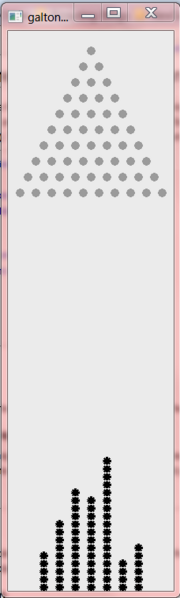
\includegraphics[scale=.6]{graphics/180px-Galtonbox-Unicon.PNG}  
\end{figure}

Example of a Galton Box at the end of animation.

In a Galton box, there are a set of pins arranged in a triangular
pattern. A number of balls are dropped so that they fall in line with
the top pin, deflecting to the left or the right of the pin. The ball
continues to fall to the left or right of subsequent pins before
arriving at one of the collection points between and to the sides of the
bottom row of pins.

For the purpose of this task the box should have at least 5 pins on the
bottom row. Your solution can use graphics or ASCII animation. Provide a
sample of the output/display such as a screenshot.

Your solution can have either one or more balls in flight at the same
time. If multiple balls are in flight, ensure they don't interfere with
each other.

Your solution should allow users to specify the number of balls or it
should run until full or a preset limit. Optionally, display the number
of balls.


\begin{wideverbatim}

(de galtonBox (Pins Height)
   (let (Bins (need (inc (* 2 Pins)) 0)  X 0  Y 0)
      (until (= Height (apply max Bins))
         (call 'clear)
         (cond
            ((=0 Y) (setq X (inc Pins)  Y 1))
            ((> (inc 'Y) Pins)
               (inc (nth Bins X))
               (zero Y) ) )
         ((if (rand T) inc dec) 'X)
         (for Row Pins
            (for Col (+ Pins Row 1)
               (let D (dec (- Col (- Pins Row)))
                  (prin
                     (cond
                        ((and (= X Col) (= Y Row)) "o")
                        ((and (gt0 D) (bit? 1 D)) ".")
                        (T " ") ) ) ) )
            (prinl) )
         (prinl)
         (for H (range Height 1)
            (for B Bins
               (prin (if (>= B H) "o" " ")) )
            (prinl) )
         (wait 200) ) ) )


\end{wideverbatim}

\begin{wideverbatim}

Test:

(galtonBox 9 11)

Output:

# Snapshot after a few seconds:
         .
        . .
       . . .
      . . . .
     . . . . .
    .o. . . . .
   . . . . . . .
  . . . . . . . .
 . . . . . . . . .

        o
        o o
      o o o o

# Final state:
         .
        . .
       . . .
      . . . .
     . . . . .
    . . . . . .
   . . . . . . .
  . . . . . . . .
 . . . . . . . . .

        o
        o
        o
        o
        o
      o o
      o o
      o o
      o o o
      o o o o o
    o o o o o o


\end{wideverbatim}




\pagebreak{}
\section*{Gamma function}

Implement one algorithm (or more) to compute the
\href{http://en.wikipedia.org/wiki/Gamma\_function}{Gamma} ($\Gamma$) function
(in the real field only). If your language has the function as builtin
or you know a library which has it, compare your implementation's
results with the results of the builtin/library function. The Gamma
function can be defined as:

\begin{figure}[htbp]
\centering
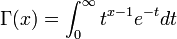
\includegraphics[scale=.6]{graphics/65e69cb6ea91c1602e057eca6ef99337.png}
% \caption{\textbackslash{}Gamma(x) =
% \textbackslash{}displaystyle\textbackslash{}int\_0\^{}\textbackslash{}infty
% t\^{}\{x-1\}e\^{}\{-t\} dt}
\end{figure}

This suggests a straightforward (but inefficient) way of computing the $\Gamma$
through numerical integration. Better suggested methods:

\begin{itemize}
\item
  \href{http://en.wikipedia.org/wiki/Lanczos\_approximation}{Lanczos
  approximation}
\item
  \href{http://en.wikipedia.org/wiki/Stirling\%27s\_approximation}{Stirling's
  approximation}
\end{itemize}


\begin{wideverbatim}

(scl 28)

(de *A
   ~(flip
      (1.00000000000000000000  0.57721566490153286061 -0.65587807152025388108
      -0.04200263503409523553  0.16653861138229148950 -0.04219773455554433675
      -0.00962197152787697356  0.00721894324666309954 -0.00116516759185906511
      -0.00021524167411495097  0.00012805028238811619 -0.00002013485478078824
      -0.00000125049348214267  0.00000113302723198170 -0.00000020563384169776
       0.00000000611609510448  0.00000000500200764447 -0.00000000118127457049
       0.00000000010434267117  0.00000000000778226344 -0.00000000000369680562
       0.00000000000051003703 -0.00000000000002058326 -0.00000000000000534812
       0.00000000000000122678 -0.00000000000000011813  0.00000000000000000119
       0.00000000000000000141 -0.00000000000000000023  0.00000000000000000002 ) ) )

(de gamma (X)
   (let (Y (- X 1.0)  Sum (car *A))
      (for A (cdr *A)
         (setq Sum (+ A (*/ Sum Y 1.0))) )
      (*/ 1.0 1.0 Sum) ) )

Output:

: (for I (range 1 10)
   (prinl (round (gamma (*/ I 1.0 3)) 14)) )
2.67893853470775
1.35411793942640
1.00000000000000
0.89297951156925
0.90274529295093
1.00000000000000
1.19063934875900
1.50457548825154
1.99999999999397
2.77815847933858

\end{wideverbatim}

\pagebreak{}
\section*{Generator}

A generator is an executable entity (like a function or procedure) that
contains code that yields a sequence of values, one at a time, so that
each time you call the generator, the next value in the sequence is
provided. Generators are often built on top of coroutines or objects so
that the internal state of the object is handled ``naturally''.
Generators are often used in situations where a sequence is potentially
infinite, and where it is possible to construct the next value of the
sequence with only minimal state.

\textbf{Task description}

\begin{enumerate}
\item
  Create a function returning a generator of the m'th powers of the
  positive integers starting from zero, in order, and without obvious or
  simple upper limit. (Any upper limit to the generator should not be
  stated in the source but should be down to factors such as the
  languages natural integer size limit or computational time/size).
\item
  Use it to create a generator of:

\begin{enumerate}
\item
  Squares.
\item
  Cubes.
\end{enumerate}

\item
  Create a new generator that filters all cubes from the generator of
  squares.
\item
  Drop the first 20 values from this last generator of filtered results
  then show the next 10 values
\end{enumerate}

Note that this task \emph{requires} the use of generators in the
calculation of the result.

\textbf{See also}

\begin{itemize}
\item
  \href{http://en.wikipedia.org/wiki/Generator\_(computer\_science)}{Generator}
\end{itemize}


\begin{wideverbatim}

Coroutines are available only in the 64-bit version.

(de powers (M)
   (co (intern (pack 'powers M))
      (for (I 0 (inc 'I))
         (yield (** I M)) ) ) )

(de filtered (N M)
   (co 'filtered
      (let (V (powers N)  F (powers M))
         (loop
            (if (> V F)
               (setq F (powers M))
               (and (> F V) (yield V))
               (setq V (powers N)) ) ) ) ) )

(do 20 (filtered 2 3))
(do 10 (println (filtered 2 3)))

Output:

529
576
625
676
784
841
900
961
1024
1089

\end{wideverbatim}

\pagebreak{}
\section*{Generic swap}

The task is to write a generic swap function or operator which exchanges
the values of two variables (or, more generally, any two storage places
that can be assigned), regardless of their types. If your solution
language is statically typed please describe the way your language
provides genericity.

If variables are typed in the given language, it is permissible that the
two variables be constrained to having a mutually compatible type, such
that each is permitted to hold the value previously stored in the other
without a type violation. That is to say, solutions do not have to be
capable of exchanging, say, a string and integer value, if the
underlying storage locations are not attributed with types that permit
such an exchange.

Generic swap is a task which brings together a few separate issues in
programming language semantics.

Dynamically typed languages deal with values in a generic way quite
readily, but do not necessarily make it easy to write a function to
destructively swap two variables, because this requires indirection upon
storage places or upon the syntax designating storage places.

Functional languages, whether static or dynamic, do not necessarily
allow a destructive operation such as swapping two variables regardless
of their generic capabilities.

Some static languages have difficulties with generic programming due
to a lack of support for (\emph{Parametric Polymorphism}).

Do your best!


\begin{wideverbatim}

[http://software-lab.de/doc/refX.html#xchg xchg] works with any data type
(let (A 1  B 2)
   (xchg 'A 'B)
   (println A B) )

(let (Lst1 '(a b c)  Lst2 '(d e f))
   (xchg (cdr Lst1) (cdr Lst2))
   (println Lst1 Lst2) )

Output:

2 1
(a e c) (d b f)

\end{wideverbatim}

\pagebreak{}
\section*{Globally replace text in several files}

The task is to replace every occuring instance of a piece of text in a
group of text files with another one. For this task we want to replace
the text ``Goodbye London!'' with ``Hello New York!'' for a list of
files.

\begin{wideverbatim}

(for File '(a.txt b.txt c.txt)
   (call 'mv File (tmp File))
   (out File
      (in (tmp File)
         (while (echo "Goodbye London!")
            (prin "Hello New York!") ) ) ) )

\end{wideverbatim}

\pagebreak{}
\section*{Go Fish}

Write a program to let the user play
\href{http://en.wikipedia.org/wiki/Go\_Fish}{Go Fish} against a
computer opponent. Use the following rules:

\begin{itemize}
\item
  Each player is dealt nine cards to start with.
\item
  On their turn, a player asks their opponent for a given rank (such as
  threes or kings). A player must already have at least one card of a
  given rank to ask for more.

  \begin{itemize}
  \item
    If the opponent has any cards of the named rank, they must hand over
    all such cards, and the requester can ask again.
  \item
    If the opponent has no cards of the named rank, the requester draws
    a card and ends their turn.
  \end{itemize}
\item
  A \emph{book} is a collection of every card of a given rank. Whenever
  a player completes a book, they may remove it from their hand.
\item
  If at any time a player's hand is empty, they may immediately draw a
  new card, so long as any new cards remain in the deck.
\item
  The game ends when every book is complete. The player with the most
  books wins.
\end{itemize}

The game's AI need not be terribly smart, but it should use at least
some strategy. That is, it shouldn't choose legal moves entirely at
random.

You may want to use code from \emph{Playing
Cards}.



\begin{wideverbatim}

(de *Ranks
   Ace 2 3 4 5 6 7 8 9 10 Jack Queen King )

(de goFish ()
   (let
      (Ocean (by '(NIL (rand)) sort (mapcan '((R) (need 4 R)) *Ranks))
         Your (cut 9 'Ocean)
         Mine (cut 9 'Ocean)
         YouHave NIL
         YouDont NIL
         YourBooks NIL
         MyBooks NIL
         Reply NIL
         Options NIL
         Request NIL )
      (loop
         (prin "Your Books: ")
         (println YourBooks)
         (prin "My Books:   ")
         (println MyBooks)
         (T (nor Your Mine Ocean)
            (let (Y (length YourBooks)  M (length MyBooks))
               (prinl
                  (cond
                     ((= Y M) "Tie game")
                     ((> Y M) "You won!")
                     (T "I won!") ) ) ) )
         (prin "You have ")
         (println Your)
         (prinl "I have " (length Mine) " cards")

\end{wideverbatim}

\begin{wideverbatim}

         (loop
            (prin
               (if Ocean
                  "Ask for a rank, lay down a book, or 'draw' a card: "
                  "Ask for a rank or lay down a book: " ) )
            (T (member (setq Reply (read)) *Ranks)
               (ifn (filter = Mine (circ Reply))
                  (prinl
                     "   I don't have any card of rank "
                     (push 'YouHave Reply) )
                  (prin "   I give you ")
                  (println @)
                  (setq
                     Mine (diff Mine @)
                     Your (append @ Your)
                     YouHave (append @ YouHave)
                     YouDont (diff YouDont @) ) ) )
            (T (and Ocean (== 'draw Reply))
               (prinl "   You draw a " (push 'Your (pop 'Ocean)))
               (off YouDont) )
            (cond
               ((atom Reply)
                  (prin "   The rank must be one of ")
                  (println *Ranks) )
               ((and (cdddr Reply) (member (car Reply) *Ranks) (not (cdr (uniq Reply))))
                  (prin "   You lay down the book ")
                  (println (push 'YourBooks Reply))
                  (setq
                     Your (diff Your Reply)
                     YouHave (diff YouHave Reply) ) )
               (T (prinl "   A book consists of four ranks, e.g. (7 7 7 7)")) ) )

\end{wideverbatim}

\begin{wideverbatim}

         (cond
            ((setq Options (diff (rot Mine) YouDont))
               (setq Request
                  (car
                     (or
                        (sect
                           (filter
                              '((Opt) (= 3 (cnt = Mine (circ Opt))))
                              Options )
                           YouHave )
                        (sect Options YouHave)
                        Options ) ) )
               (loop
                  (prin "Please give me all your " Request "s (or NIL): ")
                  (NIL (setq Reply (read))
                     (push 'YouDont Request)
                     (ifn Ocean
                        (prinl "   I pass")
                        (prinl "   I draw a card")
                        (push 'Mine (pop 'Ocean)) ) )
                  (T (and (pair Reply) (member Request Reply) (not (cdr (uniq Reply))))
                     (setq
                        Your (diff Your Reply)
                        YouHave (diff YouHave Reply)
                        Mine (append Reply Mine) ) )
                  (prinl "   I expect a list of " Request "s") ) )
            (Ocean
               (prinl "   I draw a card")
               (push 'Mine (pop 'Ocean)) )
            (T (prinl "   I pass")) )
         (while (find '((R) (= 4 (cnt = Mine (circ R)))) *Ranks)
            (let B (need 4 @)
               (prin "   I lay down the book ")
               (println (push 'MyBooks B))
               (setq Mine (diff Mine B)) ) )
         (prinl) ) ) )

\end{wideverbatim}

\pagebreak{}
\section*{Gray code}

\href{http://en.wikipedia.org/wiki/Gray\_code}{Gray code} is a form of
binary encoding where transitions between consecutive numbers differ by
only one bit. This is a useful encoding for reducing hardware data
hazards with values that change rapidly and/or connect to slower
hardware as inputs. It is also useful for generating inputs for
\href{http://en.wikipedia.org/wiki/Karnaugh\_map}{Karnaugh maps} in
order from left to right or top to bottom.

Create functions to encode a number to and decode a number from Gray
code. Display the normal binary representations, Gray code
representations, and decoded Gray code values for all 5-bit binary
numbers (0-31 inclusive, leading 0's not necessary).

There are many possible Gray codes. The following encodes what is called
``binary reflected Gray code.''

Encoding (MSB is bit 0, b is binary, g is Gray code):

\begin{verbatim}
if b[i-1] = 1
   g[i] = not b[i]
else
   g[i] = b[i]
\end{verbatim}

Or:

\begin{verbatim}
g = b xor (b logically right shifted 1 time)
\end{verbatim}

Decoding (MSB is bit 0, b is binary, g is Gray code):

\begin{verbatim}
b[0] = g[0]

for other bits:
b[i] = g[i] xor b[i-1]
\end{verbatim}

Reference

\begin{itemize}
\item
  \href{http://www.wisc-online.com/Objects/ViewObject.aspx?ID=IAU8307}{Converting
  Between Gray and Binary Codes}. It includes step-by-step animations.
\end{itemize}



\begin{wideverbatim}

(de grayEncode (N)
   (bin (x| N (>> 1 N))) )

(de grayDecode (G)
   (bin
      (pack
         (let X 0
            (mapcar
               '((C) (setq X (x| X (format C))))
               (chop G) ) ) ) ) )

Test:

(prinl "       Binary     Gray  Decoded")
(for I (range 0 31)
   (let G (grayEncode I)
      (tab (4 9 9 9) I (bin I) G (grayDecode G)) ) )

Output:

       Binary     Gray  Decoded
   0        0        0        0
   1        1        1        1
   2       10       11        2
   3       11       10        3
   4      100      110        4
   5      101      111        5
   6      110      101        6
   7      111      100        7
   8     1000     1100        8
   9     1001     1101        9
  10     1010     1111       10
  11     1011     1110       11
  12     1100     1010       12
  13     1101     1011       13
  14     1110     1001       14
  15     1111     1000       15
  16    10000    11000       16
  17    10001    11001       17
  18    10010    11011       18
  19    10011    11010       19
  20    10100    11110       20
  21    10101    11111       21
  22    10110    11101       22
  23    10111    11100       23
  24    11000    10100       24
  25    11001    10101       25
  26    11010    10111       26
  27    11011    10110       27
  28    11100    10010       28
  29    11101    10011       29
  30    11110    10001       30
  31    11111    10000       31

\end{wideverbatim}

\pagebreak{}
\section*{Grayscale image}

Many image processing algorithms are defined for
\href{http://en.wikipedia.org/wiki/Grayscale}{grayscale} (or else
monochromatic) images. Extend the data storage type defined \emph{on
  this page} to support grayscale images. Define two operations, one
to convert a color image to a grayscale image and one for the backward
conversion. To get luminance of a color use the formula recommended by
\href{http://www.cie.co.at/index\_ie.html}{CIE}:

\begin{verbatim}
L = 0.2126·R + 0.7152·G + 0.0722·B
\end{verbatim}

When using floating-point arithmetic make sure that rounding errors
would not cause run-time problems or else distorted results when
calculated luminance is stored as an unsigned integer.

\begin{wideverbatim}

# Convert color image (PPM) to greyscale image (PGM)
(de ppm->pgm (Ppm)
   (mapcar
      '((Y)
         (mapcar
            '((C)
               (/
                  (+
                     (* (car C) 2126)  # Red
                     (* (cadr C) 7152)  # Green
                     (* (caddr C) 722) )  # Blue
                  10000 ) )
            Y ) )
      Ppm ) )

# Convert greyscale image (PGM) to color image (PPM)
(de pgm->ppm (Pgm)
   (mapcar
      '((Y)
         (mapcar
            '((G) (list G G G))
            Y ) )
      Pgm ) )

# Write greyscale image (PGM) to file
(de pgmWrite (Pgm File)
   (out File
      (prinl "P5")
      (prinl (length (car Pgm)) " " (length Pgm))
      (prinl 255)
      (for Y Pgm (apply wr Y)) ) )

# Create an empty image of 120 x 90 pixels
(setq *Ppm (make (do 90 (link (need 120)))))

# Fill background with green color
(ppmFill *Ppm 0 255 0)

# Draw a diagonal line
(for I 80 (ppmSetPixel *Ppm I I 0 0 0))


# Convert to greyscale image (PGM)
(setq *Pgm (ppm->pgm *Ppm))

# Write greyscale image to .pgm file
(pgmWrite *Pgm "img.pgm")

# Convert to color image and write to .ppm file
(ppmWrite (pgm->ppm *Pgm) "img.ppm")

\end{wideverbatim}

\pagebreak{}
\section*{Greatest common divisor}

This task requires the finding of the greatest common divisor of two
integers.

\begin{wideverbatim}

(de gcd (A B)
   (until (=0 B)
      (let M (\% A B)
         (setq A B B M) ) )
   (abs A) )

\end{wideverbatim}

\pagebreak{}
\section*{Greatest element of a list}

Create a function that returns the maximum value in a provided set of
values, where the number of values may not be known until runtime.

\begin{wideverbatim}

: (max 2 4 1 3)               # Return the maximal argument
-> 4
: (apply max (2 4 1 3))       # Apply to a list
-> 4
: (maxi abs (2 -4 -1 3))      # Maximum according to given function
-> -4

\end{wideverbatim}

\pagebreak{}
\section*{Greatest subsequential sum}

Given a sequence of integers, find a continuous subsequence which
maximizes the sum of its elements, that is, the elements of no other
single subsequence add up to a value larger than this one. An empty
subsequence is considered to have the sum 0; thus if all elements are
negative, the result must be the empty sequence.


\begin{wideverbatim}

(maxi '((L) (apply + L))
   (mapcon '((L) (maplist reverse (reverse L)))
      (-1 -2 3 5 6 -2 -1 4 -4 2 -1) ) )

Output:

-> (3 5 6 -2 -1 4)

\end{wideverbatim}


\pagebreak{}
\section*{Greyscale bars/Display}

The task is to display a series of vertical greyscale bars (contrast
bars) with a sufficient number of bars to span the entire width of the
display.

For the top quarter of the display, the left hand bar should be black,
and we then incrementally step through six shades of grey until we have
a white bar on the right hand side of the display. (This gives a total
of 8 bars)

For the second quarter down, we start with white and step down through
14 shades of gray, getting darker until we have black on the right hand
side of the display. (This gives a total of 16 bars).

Halfway down the display, we start with black, and produce 32 bars,
ending in white, and for the last quarter, we start with white and step
through 62 shades of grey, before finally arriving at black in the
bottom right hand corner, producing a total of 64 bars for the bottom
quarter.


\begin{wideverbatim}

(let Pgm  # Create PGM of 384 x 288 pixels
   (make
      (for N 4
         (let L
            (make
               (for I (* N 8)
                  (let C (*/ (dec I) 255 (dec (* N 8)))
                     (unless (bit? 1 N)
                        (setq C (- 255 C)) )
                     (do (/ 48 N) (link C)) ) ) )
            (do 72 (link L)) ) ) )
   (out '(display)  # Pipe to ImageMagick
      (prinl "P5")  # NetPBM format
      (prinl (length (car Pgm)) " " (length Pgm))
      (prinl 255)
      (for Y Pgm (apply wr Y)) ) )

\end{wideverbatim}


\pagebreak{}
\section*{Guess the number}

The task is to write a program where the program chooses a number
between 1 and 10. A player is then prompted to enter a guess. If the
player guess wrong then the prompt appears again until the guess is
correct. When the player has made a successful guess the computer will
give a ``Well guessed!'' message, and the program will exit.

A \emph{conditional loop} may be used to repeat the guessing until the
user is correct.

Cf. \emph{Guess the number/With Feedback}, \emph{Bulls and cows}


\begin{wideverbatim}

(de guessTheNumber ()
   (let Number (rand 1 9)
      (loop
         (prin "Guess the number: ")
         (T (= Number (read))
            (prinl "Well guessed!") )
         (prinl "Sorry, this was wrong") ) ) )

\end{wideverbatim}

\pagebreak{}
\section*{Guess the number/With Feedback}

The task is to write a game that follows the following rules:

The computer will choose a number between given set limits and asks the
player for repeated guesses until the player guesses the target number
correctly. At each guess, the computer responds with whether the guess
was higher than, equal to, or less than the target - or signals that the
input was inappropriate.

C.f: \emph{Guess the number/With Feedback (Player)}

\begin{wideverbatim}

(de guessTheNumber ()
   (use (Low High Guess)
      (until
         (and
            (prin "Enter low limit : ")
            (setq Low (read))
            (prin "Enter high limit: ")
            (setq High (read))
            (> High Low) ) )
      (seed (time))
      (let Number (rand Low High)
         (loop
            (prin "Guess what number I have: ")
            (T (= Number (setq Guess (read)))
               (prinl "You got it!") )
            (prinl
               "Your guess is too "
               (if (> Number Guess) "low" "high")
               "." ) ) ) ) )

Output:

: (guessTheNumber)
Enter low limit : 1
Enter high limit: 64
Guess what number I have: 32
Your guess is too high.
Guess what number I have: 16
Your guess is too low.
Guess what number I have: 24
You got it!

\end{wideverbatim}

\pagebreak{}
\section*{Guess the number/With Feedback (Player)}

The task is to write a player for the game that follows the following
rules:

The scorer will choose a number between set limits. The computer player
will print a guess of the target number. The computer asks for a score
of whether its guess is higher than, lower than, or equal to the target.
The computer guesses, and the scorer scores, in turn, until the computer
correctly guesses the target number.

The computer should guess intelligently based on the accumulated scores
given. One way is to use a \emph{Binary search}
based algorithm.

Cf.

\begin{itemize}
\item
  \emph{Guess the number/With
  Feedback}
\item
  \emph{Bulls and cows/Player}
\end{itemize}


\begin{wideverbatim}

(de guessTheNumber (Min Max)
   (prinl "Think of a number between " Min " and " Max ".")
   (prinl "On every guess of mine you should state whether my guess was")
   (prinl "too high, too low, or equal to your number by typing 'h', 'l', Or '='")
   (use Guess
      (loop
         (NIL (> Max Min)
            (prinl "I think somthing is strange here...") )
         (prin
            "My guess is "
            (setq Guess (+ Min (/ (- Max Min) 2)))
            ",is this correct? " )
         (flush)
         (NIL
            (case (uppc (car (line)))
               ("H" (setq Max Guess))
               ("L" (setq Min Guess))
               ("=" (nil (prinl "I did it!")))
               (T (prinl "I do not understand that...")) ) ) ) ) )

Output:

: (guessTheNumber 1 99)
Think of a number between 1 and 99.
On every guess of mine you should state whether my guess was
too high, too low, or equal to your number by typing 'h', 'l', Or '='
My guess is 50,is this correct? h
My guess is 25,is this correct? h
My guess is 13,is this correct? l
My guess is 19,is this correct? l
My guess is 22,is this correct? =
I did it!

\end{wideverbatim}



% %%%%%%%%%%%%%%%%%%%%%%%% referenc.tex %%%%%%%%%%%%%%%%%%%%%%%%%%%%%%
% sample references
% %
% Use this file as a template for your own input.
%
%%%%%%%%%%%%%%%%%%%%%%%% Springer-Verlag %%%%%%%%%%%%%%%%%%%%%%%%%%
%
% BibTeX users please use
% \bibliographystyle{}
% \bibliography{}
%
\biblstarthook{In view of the parallel print and (chapter-wise) online publication of your book at \url{www.springerlink.com} it has been decided that -- as a genreral rule --  references should be sorted chapter-wise and placed at the end of the individual chapters. However, upon agreement with your contact at Springer you may list your references in a single seperate chapter at the end of your book. Deactivate the class option \texttt{sectrefs} and the \texttt{thebibliography} environment will be put out as a chapter of its own.\\\indent
References may be \textit{cited} in the text either by number (preferred) or by author/year.\footnote{Make sure that all references from the list are cited in the text. Those not cited should be moved to a separate \textit{Further Reading} section or chapter.} The reference list should ideally be \textit{sorted} in alphabetical order -- even if reference numbers are used for the their citation in the text. If there are several works by the same author, the following order should be used: 
\begin{enumerate}
\item all works by the author alone, ordered chronologically by year of publication
\item all works by the author with a coauthor, ordered alphabetically by coauthor
\item all works by the author with several coauthors, ordered chronologically by year of publication.
\end{enumerate}
The \textit{styling} of references\footnote{Always use the standard abbreviation of a journal's name according to the ISSN \textit{List of Title Word Abbreviations}, see \url{http://www.issn.org/en/node/344}} depends on the subject of your book:
\begin{itemize}
\item The \textit{two} recommended styles for references in books on \textit{mathematical, physical, statistical and computer sciences} are depicted in ~\cite{science-contrib, science-online, science-mono, science-journal, science-DOI} and ~\cite{phys-online, phys-mono, phys-journal, phys-DOI, phys-contrib}.
\item Examples of the most commonly used reference style in books on \textit{Psychology, Social Sciences} are~\cite{psysoc-mono, psysoc-online,psysoc-journal, psysoc-contrib, psysoc-DOI}.
\item Examples for references in books on \textit{Humanities, Linguistics, Philosophy} are~\cite{humlinphil-journal, humlinphil-contrib, humlinphil-mono, humlinphil-online, humlinphil-DOI}.
\item Examples of the basic Springer style used in publications on a wide range of subjects such as \textit{Computer Science, Economics, Engineering, Geosciences, Life Sciences, Medicine, Biomedicine} are ~\cite{basic-contrib, basic-online, basic-journal, basic-DOI, basic-mono}. 
\end{itemize}
}

\begin{thebibliography}{99.}%
% and use \bibitem to create references.
%
% Use the following syntax and markup for your references if 
% the subject of your book is from the field 
% "Mathematics, Physics, Statistics, Computer Science"
%
% Contribution 
\bibitem{science-contrib} Broy, M.: Software engineering --- from auxiliary to key technologies. In: Broy, M., Dener, E. (eds.) Software Pioneers, pp. 10-13. Springer, Heidelberg (2002)
%
% Online Document
\bibitem{science-online} Dod, J.: Effective substances. In: The Dictionary of Substances and Their Effects. Royal Society of Chemistry (1999) Available via DIALOG. \\
\url{http://www.rsc.org/dose/title of subordinate document. Cited 15 Jan 1999}
%
% Monograph
\bibitem{science-mono} Geddes, K.O., Czapor, S.R., Labahn, G.: Algorithms for Computer Algebra. Kluwer, Boston (1992) 
%
% Journal article
\bibitem{science-journal} Hamburger, C.: Quasimonotonicity, regularity and duality for nonlinear systems of partial differential equations. Ann. Mat. Pura. Appl. \textbf{169}, 321--354 (1995)
%
% Journal article by DOI
\bibitem{science-DOI} Slifka, M.K., Whitton, J.L.: Clinical implications of dysregulated cytokine production. J. Mol. Med. (2000) doi: 10.1007/s001090000086 
%
\bigskip

% Use the following (APS) syntax and markup for your references if 
% the subject of your book is from the field 
% "Mathematics, Physics, Statistics, Computer Science"
%
% Online Document
\bibitem{phys-online} J. Dod, in \textit{The Dictionary of Substances and Their Effects}, Royal Society of Chemistry. (Available via DIALOG, 1999), 
\url{http://www.rsc.org/dose/title of subordinate document. Cited 15 Jan 1999}
%
% Monograph
\bibitem{phys-mono} H. Ibach, H. L\"uth, \textit{Solid-State Physics}, 2nd edn. (Springer, New York, 1996), pp. 45-56 
%
% Journal article
\bibitem{phys-journal} S. Preuss, A. Demchuk Jr., M. Stuke, Appl. Phys. A \textbf{61}
%
% Journal article by DOI
\bibitem{phys-DOI} M.K. Slifka, J.L. Whitton, J. Mol. Med., doi: 10.1007/s001090000086
%
% Contribution 
\bibitem{phys-contrib} S.E. Smith, in \textit{Neuromuscular Junction}, ed. by E. Zaimis. Handbook of Experimental Pharmacology, vol 42 (Springer, Heidelberg, 1976), p. 593
%
\bigskip
%
% Use the following syntax and markup for your references if 
% the subject of your book is from the field 
% "Psychology, Social Sciences"
%
%
% Monograph
\bibitem{psysoc-mono} Calfee, R.~C., \& Valencia, R.~R. (1991). \textit{APA guide to preparing manuscripts for journal publication.} Washington, DC: American Psychological Association.
%
% Online Document
\bibitem{psysoc-online} Dod, J. (1999). Effective substances. In: The dictionary of substances and their effects. Royal Society of Chemistry. Available via DIALOG. \\
\url{http://www.rsc.org/dose/Effective substances.} Cited 15 Jan 1999.
%
% Journal article
\bibitem{psysoc-journal} Harris, M., Karper, E., Stacks, G., Hoffman, D., DeNiro, R., Cruz, P., et al. (2001). Writing labs and the Hollywood connection. \textit{J Film} Writing, 44(3), 213--245.
%
% Contribution 
\bibitem{psysoc-contrib} O'Neil, J.~M., \& Egan, J. (1992). Men's and women's gender role journeys: Metaphor for healing, transition, and transformation. In B.~R. Wainrig (Ed.), \textit{Gender issues across the life cycle} (pp. 107--123). New York: Springer.
%
% Journal article by DOI
\bibitem{psysoc-DOI}Kreger, M., Brindis, C.D., Manuel, D.M., Sassoubre, L. (2007). Lessons learned in systems change initiatives: benchmarks and indicators. \textit{American Journal of Community Psychology}, doi: 10.1007/s10464-007-9108-14.
%
%
% Use the following syntax and markup for your references if 
% the subject of your book is from the field 
% "Humanities, Linguistics, Philosophy"
%
\bigskip
%
% Journal article
\bibitem{humlinphil-journal} Alber John, Daniel C. O'Connell, and Sabine Kowal. 2002. Personal perspective in TV interviews. \textit{Pragmatics} 12:257--271
%
% Contribution 
\bibitem{humlinphil-contrib} Cameron, Deborah. 1997. Theoretical debates in feminist linguistics: Questions of sex and gender. In \textit{Gender and discourse}, ed. Ruth Wodak, 99--119. London: Sage Publications.
%
% Monograph
\bibitem{humlinphil-mono} Cameron, Deborah. 1985. \textit{Feminism and linguistic theory.} New York: St. Martin's Press.
%
% Online Document
\bibitem{humlinphil-online} Dod, Jake. 1999. Effective substances. In: The dictionary of substances and their effects. Royal Society of Chemistry. Available via DIALOG. \\
http://www.rsc.org/dose/title of subordinate document. Cited 15 Jan 1999
%
% Journal article by DOI
\bibitem{humlinphil-DOI} Suleiman, Camelia, Daniel C. O�Connell, and Sabine Kowal. 2002. `If you and I, if we, in this later day, lose that sacred fire...�': Perspective in political interviews. \textit{Journal of Psycholinguistic Research}. doi: 10.1023/A:1015592129296.
%
%
%
\bigskip
%
%
% Use the following syntax and markup for your references if 
% the subject of your book is from the field 
% "Computer Science, Economics, Engineering, Geosciences, Life Sciences"
%
%
% Contribution 
\bibitem{basic-contrib} Brown B, Aaron M (2001) The politics of nature. In: Smith J (ed) The rise of modern genomics, 3rd edn. Wiley, New York 
%
% Online Document
\bibitem{basic-online} Dod J (1999) Effective Substances. In: The dictionary of substances and their effects. Royal Society of Chemistry. Available via DIALOG. \\
\url{http://www.rsc.org/dose/title of subordinate document. Cited 15 Jan 1999}
%
% Journal article by DOI
\bibitem{basic-DOI} Slifka MK, Whitton JL (2000) Clinical implications of dysregulated cytokine production. J Mol Med, doi: 10.1007/s001090000086
%
% Journal article
\bibitem{basic-journal} Smith J, Jones M Jr, Houghton L et al (1999) Future of health insurance. N Engl J Med 965:325--329
%
% Monograph
\bibitem{basic-mono} South J, Blass B (2001) The future of modern genomics. Blackwell, London 
%
\end{thebibliography}

